\documentclass[reprint,amsmath,amssymb,aps,]{revtex4-2}
\usepackage{graphicx}
\usepackage{dcolumn}
\usepackage{bm}
\usepackage{scrextend}
\usepackage{vmargin}
\usepackage{multirow}
\usepackage[utf8]{inputenc}
\usepackage[spanish, es-tabla]{babel}
\usepackage{enumerate}
\usepackage{float}
\usepackage{lipsum}
\usepackage{caption}
\usepackage{subcaption}
\usepackage{amsmath, amsthm, amssymb, amsfonts}
\usepackage[usenames]{color}
\usepackage[breaklinks=true,hidelinks]{hyperref}
\pagestyle{empty}
\begin{document}
\preprint{APS/123-QED}
\begin{abstract}
Se propuso un sistema conformado por átomos de carbono en dos y tres dimensiones en los cuales se vario sus densidades en diferentes valores
, los sistemas se dejaran interaccionar en una simulación bajo
el efecto del potencial de Lennard-Jones realizando 2x$10^{6}$ pasos. Durante la simulación se monitoreo la energía
cinética, energía potencial y energía total, a la par se calculó su función de distribución radial de los sistemas.\\
\textbf{Palabras clave:} Potencial de Lennard-Jones, distribución radial, dos dimensiones
\end{abstract}
\begin{titlepage}
\begin{center}

\includegraphics[scale=0.40]{../../../Logos/uanl.png} 
\hspace{2.5cm}

\includegraphics[scale=0.40]{../../../Logos/fcfm.png}
\end{center}
\vspace{2cm}
\begin{center}
\textbf{
UNIVERSIDAD AUTÓNOMA DE NUEVO LEÓN\\
FACULTAD DE CIENCIAS
FÍSICO MATEMÁTICAS}\\
\vspace*{2cm}
\begin{large}
\vspace{1cm}
\textbf{Simuladores Moleculares\vspace{0.5cm}\\
Dinámica molecular con el potencial \\ de Lennard-Jones en dos y tres dimensiones\\ para diferntes densidades}\\
Omar Gonzalez Amezcua\\
\end{large}
\vspace{3.5cm}
\begin{minipage}{0.6\linewidth}
\vspace{0.5cm}
\changefontsizes{14pt}
Nombre:\\
Giovanni Gamaliel López Padilla\\
\end{minipage}
\begin{minipage}{0.2\linewidth}
\changefontsizes{14pt}
Matricula:\\
1837522
\end{minipage}
\end{center}
\vspace{4cm}
\begin{flushright}
\today
\end{flushright}
\pagebreak
\end{titlepage}
\maketitle
\section{Introducción}
\section{Objetivo general}
 \section{Objetivo específico}
\section{Marco teórico}
El potencial de Lennard-Jones describe la energía potencial de interacción entre dos átomos o moleculas netros sujetos a dos fuerzas distintas, una fuerza que tiene mayor acción cuando la distancia entre las dos sistemas es grande y la otra fuerza de interacción tiene una mayor acción a corta distancia. Este potencial tiene la siguiente forma:
\begin{equation}
    \label{Potencial de Lennard-Jones}
    V(r) = 4 \epsilon \left[\left(\frac{\sigma}{r} \right)^{12} - \left(\frac{\sigma}{r} \right)^6 \right]
\end{equation}
donde:
\begin{itemize}
    \item $V$ es el potencial intermolecular entre dos átomos o partículas.
    \item $\epsilon$ es la profundidad del valle que define que tan fuerte es la atracción entre partículas.
    \item $\sigma$ es la distancia a la cual el potencial entre dos partículas es igual a cero.
    \item $r$ es la distancia de separación entre dos partículas
\end{itemize}
Los parámetros $\epsilon$ y $\sigma$ son ajustados para reproducir datos experimentales o pueden ser dedudidos de resultados a partir de cálculos de química cuántica. La fígura \ref{Potencial de Lennard-Jones} es el potencial de Lennard-Jones con $\epsilon=1$ y $\sigma=1$.\\
En donde expone una gráfica de potenciales universales para estructuras de gráfito, y la que tenemos se asemeja en comportamiento a pesar de no tener la estrucura de un grafito.
Teniendo el potencial de la ecuación \ref{Potencial de Lennard-Jones}, podemos deducir la fuerza, ya que esta puede ser deducida a partir de aplicar el gradiente a la función $V(r)$, teniendo así la siguiente expresión:
\begin{equation}
    \label{eq:fuerzateo}
    \vec{F}(r)= 48\epsilon \left(\frac{\sigma^{12}}{r^{13}}- \frac{1}{2}\frac{\sigma^6}{r^7} \right) \hat{r}
\end{equation}
\begin{figure}[H]
    \centering
    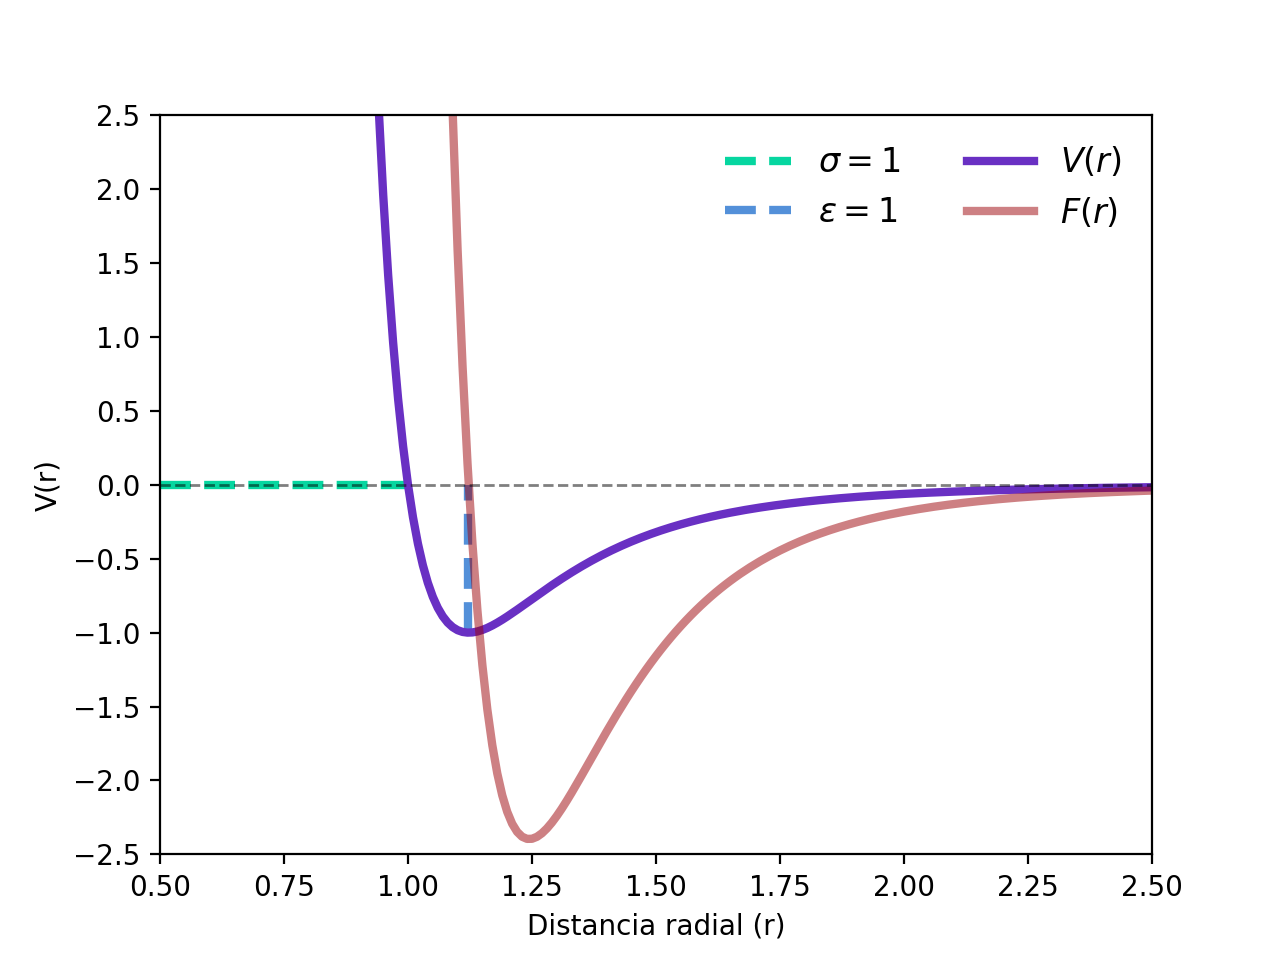
\includegraphics[scale=0.45]{../Graphics/Potencial.png}
    \caption{Potencial y fuerza de Lennard-Jones}
    \label{pot-len-jones}
\end{figure}
\begin{table*}
    \centering
    \begin{tabular}{ccp{1cm}p{0.5cm}cc}
        \hline
        Dimensión & Número de átomos & $\epsilon$ & $\sigma $ & $\rho $ & Número de pasos \\ \hline
        2 &784 &\multirow{2}{*}{1} &\multirow{2}{*}{1}  &\multirow{2}{*}{Variable$^{*}$}  &\multirow{2}{*}{$2x10^{6}$}  \\
        3 &864 & & & & \\ \hline
    \end{tabular}
    \caption{Parámetros para la simulación para las diferentes dimensiones.}
    \label{table:parametros}
\end{table*}
reescribiendo las ecuaciones \ref{Potencial de Lennard-Jones} y \ref{eq:fuerzateo} para tener la suma de estas en un sistema de n particulas se tiene lo siguiente:
\begin{equation}
    \label{eq:pot-n}
    U_t=\left\langle\sum_{i=1}^N \sum_{j<i}^N V_i,j(|r_j-r_i|)\right\rangle_t
\end{equation}
\begin{equation}
    \changefontsizes{9pt}
    \label{eq:f-n}
    F_i = \frac{48}{\sigma^2} \sum_{j \ne i} \left[\left(\frac{\sigma}{r_{ij}}\right)^{14}-\frac{1}{2}\left(\frac{\sigma}{r_{ij}} \right)^8  \right] (r_j-r_i)
\end{equation}
Teniendo ya la dinámica se este sistema podemos ir monitoreando la energía cinética de la siguiente manera:
\begin{equation}
    \label{eq:kin-n}
    T_t=\left\langle \sum_{i=1}^N \frac{1}{2}m|v_i(t)|^2\right\rangle
\end{equation}
por lo tanto, la energía total para un tiempo t será:
\begin{equation}
    \label{eq:e-tot}
    E_t=T_t+U_t
\end{equation}
\section{Resultados}
\begin{figure*}
    \hspace*{-2cm}
    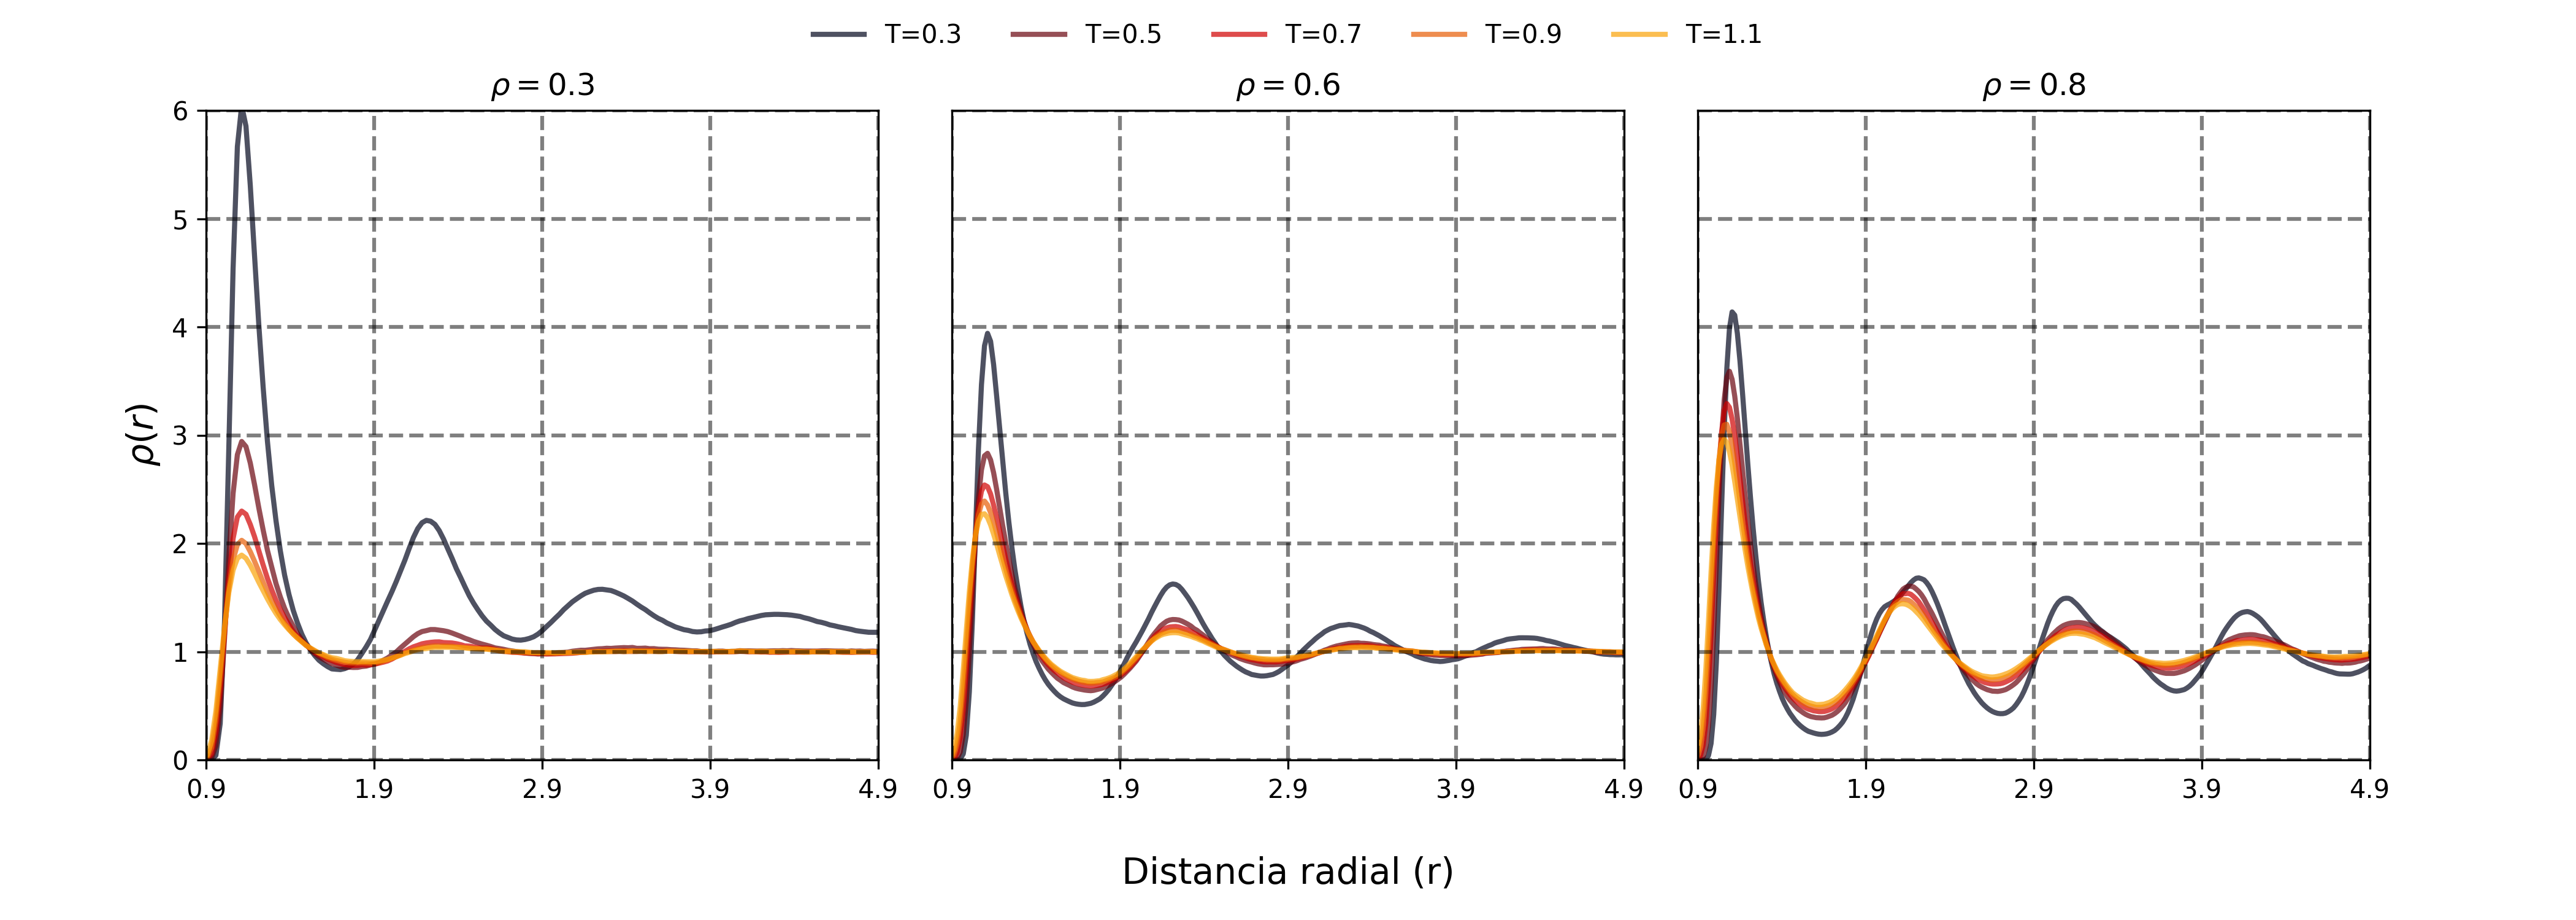
\includegraphics[scale=0.53]{../Graphics/Dis_rad.png}
    \caption{Distribución radial de la estructura}
    \label{eq:disradial}
\end{figure*}
\begin{figure*}
    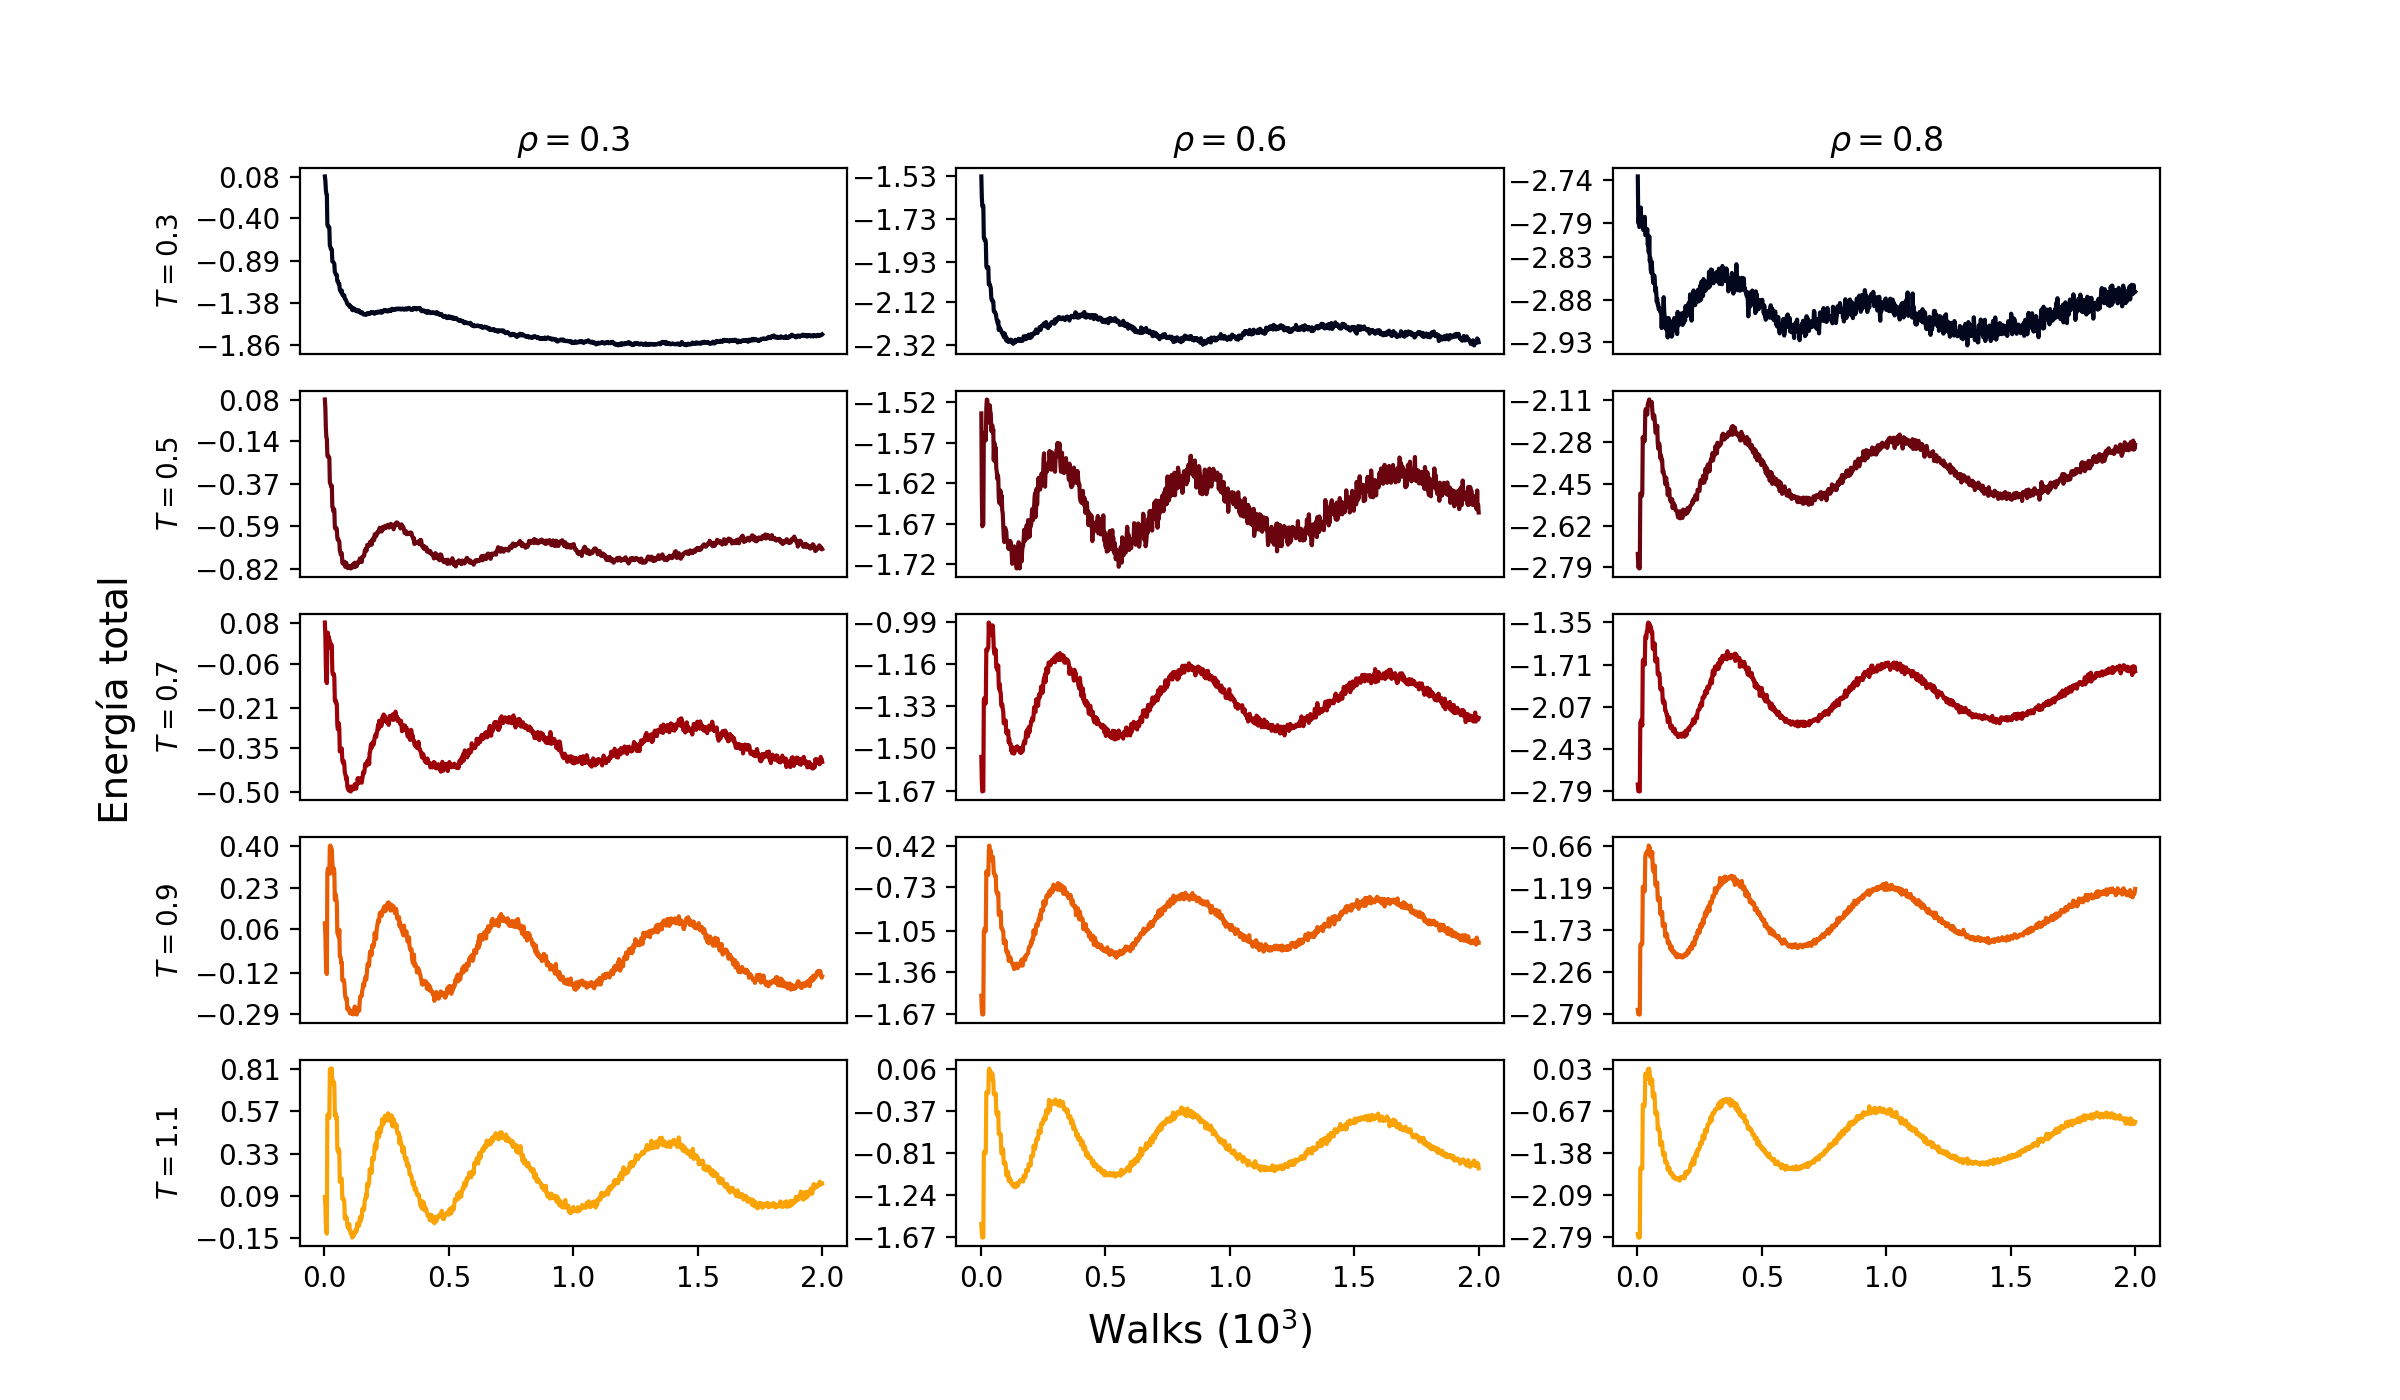
\includegraphics[scale=0.53]{../Graphics/Energy.png}
    \caption{Energía total a lo largo de la simulación de las densidades seleccionadas variando la temperadura del exterior.}
\end{figure*}
\section{Código}
\bibliographystyle{plain}
\nocite{*}
\bibliography{Main}
\end{document}